\documentclass[onecolumn, 11pt,openany]{memoir}

% packages
\usepackage{blindtext, color}
\usepackage[usenames,dvipsnames,svgnames,table,xcdraw]{xcolor}
\usepackage{graphicx}  
\usepackage{import}  
\usepackage[english]{babel}
\usepackage[outline]{contour} 
\usepackage{ctable}
\newcolumntype{d}[1]{D{.}{.}{#1}}
\usepackage[utf8]{inputenc}
\usepackage[compact]{titlesec}
\usepackage{pdfpages}
\usepackage{float}
\usepackage{microtype}
\definecolor{lightgray}{gray}{0.9}
\usepackage{multicol}
\usepackage{authblk}

% font and lay-out
%current font: BT Charter. Find other fonts at http://www.tug.dk/FontCatalogue/
\usepackage[bitstream-charter]{mathdesign}
\usepackage[T1]{fontenc}

%caption layout
\usepackage[format=plain]{caption}
\DeclareCaptionLabelSeparator{bar}{ | }
\captionsetup[figure]{labelfont={bf},name={Figure},labelsep=bar,font=footnotesize}
\captionsetup[table]{labelfont={bf},name={Table},labelsep=bar,font=footnotesize}

%symbols
\usepackage{textcomp}
\usepackage{gensymb}
\usepackage[euler]{textgreek}

% paragraph indent & spacing
\setlength\parskip{\baselineskip}
\setlength\parindent{0pt} % use 0 pt for no indent

% page sizes and margins
\usepackage[a4paper, margin=1in]{geometry}

% dummy text; just for testing
\usepackage{lipsum}

% hyphenation
% list all hy-phe-na-ted words as they should be hyphenated
% to repress hyphenation place word (or two) in an mbox operator; e.g.:  \mbox{P. infestans} 

\hyphenation{hy-phe-na-te}

\label{START}
\begin{document}
\thispagestyle{empty}                   
\frontmatter

\title{Preprinting your latest ground-breaking research}
\author[1,2]{Author 1}
\author[1]{Author 2}
\author[3]{Author 3}
\begin{scriptsize}
\affil[1]{University 1}
\affil[2]{University 2}
\affil[3]{University 3}
\end{scriptsize}
\date{\vspace{-5ex}} % this is workaround to remove date and move main text up. For printing date remove vspace operator
\maketitle

\subsection{Correspondence}
firstname.lastname@univ.edu

\pagenumbering{arabic}
\pagestyle{plain}

\section{Abstract}
\lipsum[1-1]

\begin{multicols}{2}
\section{Introduction}
\lipsum[2-5]

\section{Results}
\subsection{Experiment 1}
\lipsum[6-8]

%figure referencing as following. Remove \textbf operator to print links not bold
These data show us that we successfully silenced our favourite gene \textbf{Figure ~\ref{fig1}}. All individual measurements are listed in \textbf{Table ~\ref{tabS1_measurements}}.

\begin{figure*}[t]
\centering
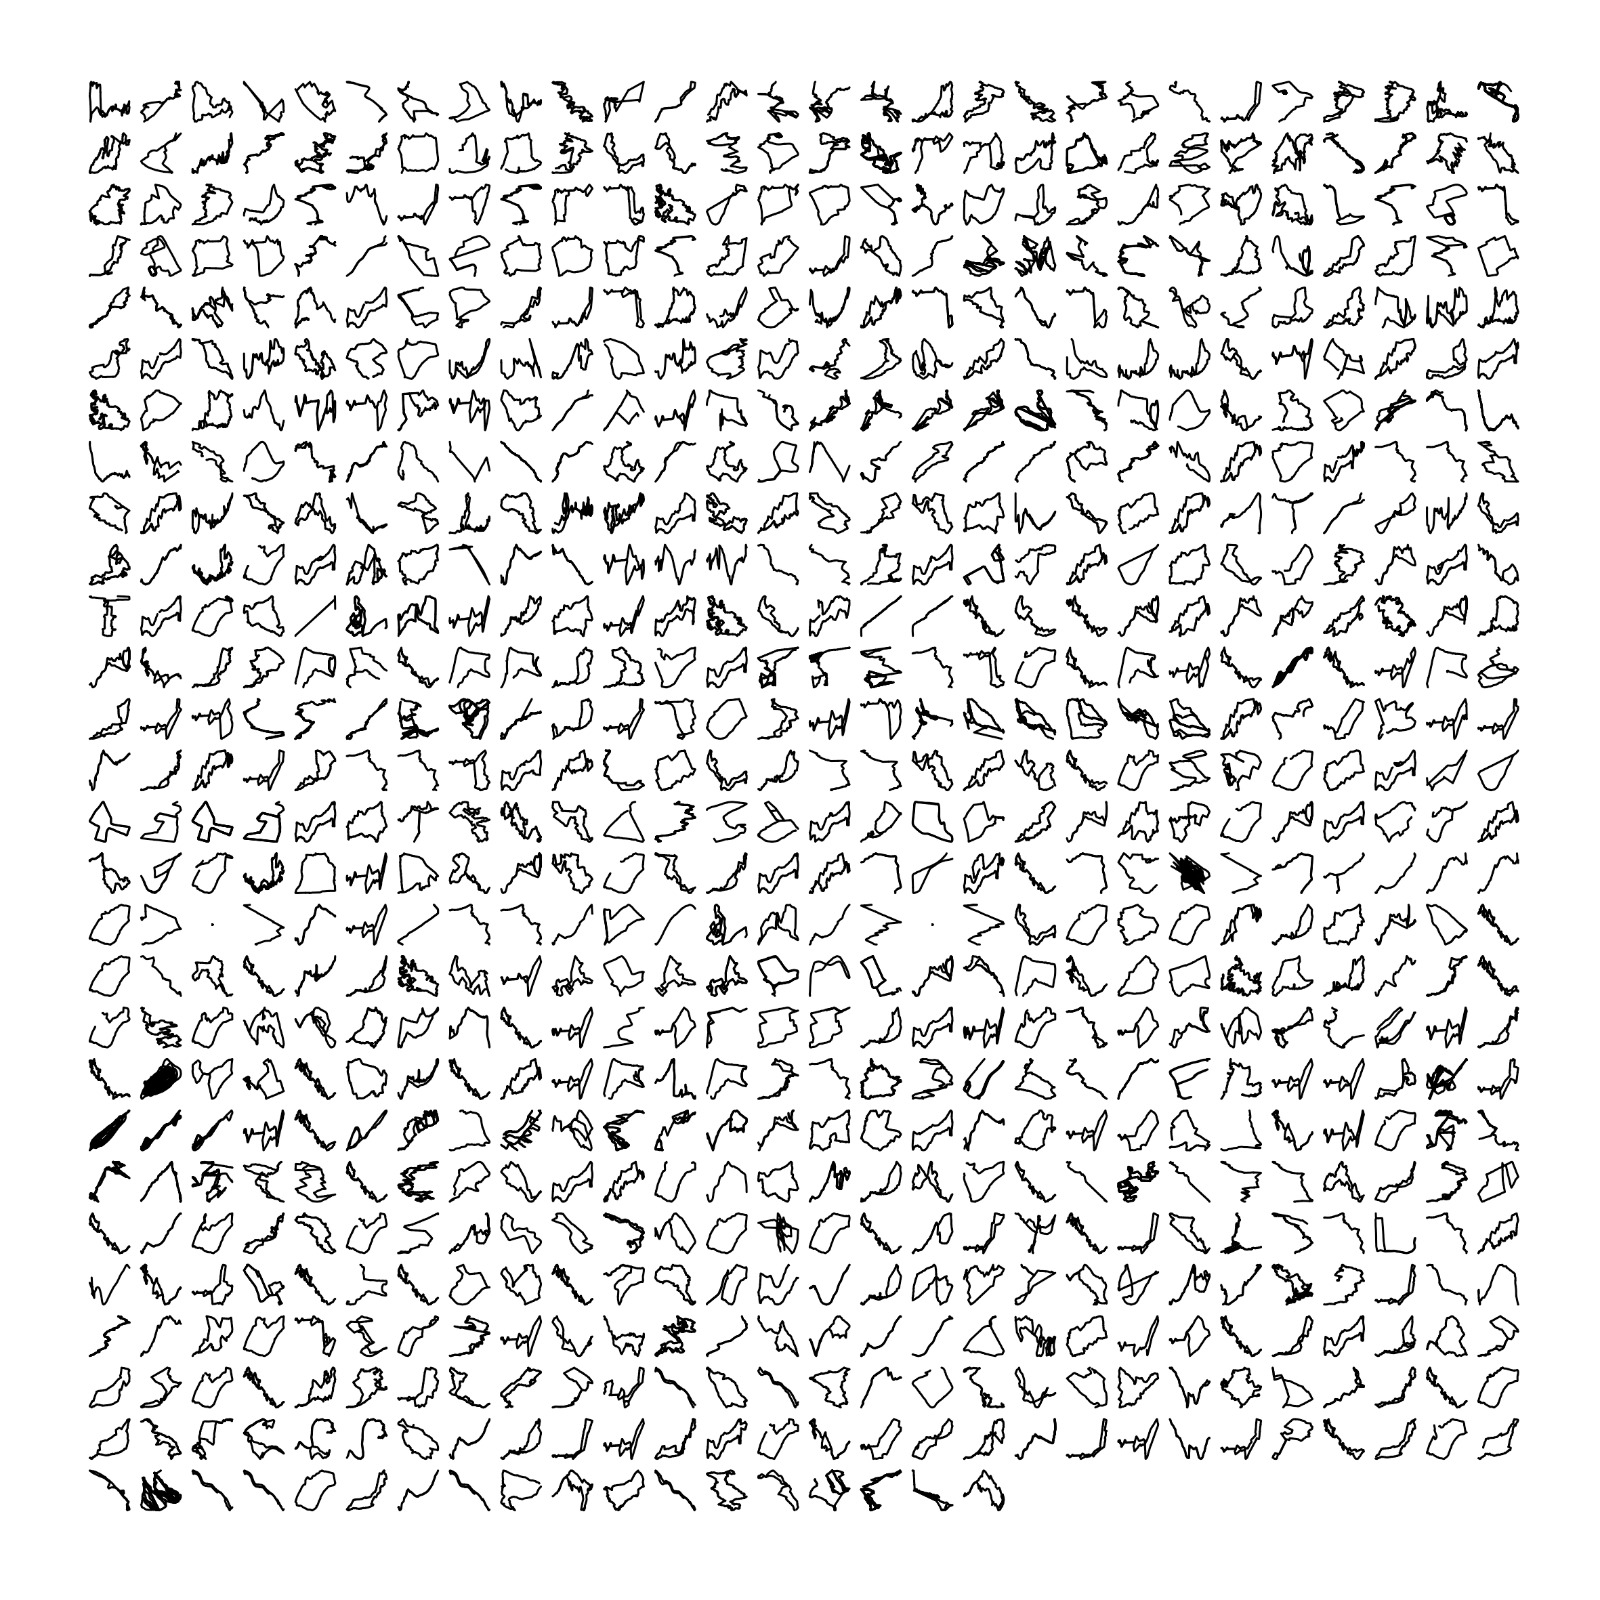
\includegraphics[width=1\textwidth]{Figures/Fig1}
\caption{\textbf{CRISPR loci and HDR constructs.} \textbf{(a)} \textit{PiAvr1}, \textbf{(b) }\textit{PiTubA1}, and \textbf{(c)} \textit{PiAP5}. Orange arrowheads indicate expected DSB sites upon Cas9 nuclease activity; black arrows indicate start codons (ATG); grey blocks mark homologous regions between the genes and the HDR constructs (referred to as repair template or ssODN); interpuncts (•) represent cropped sequences; PAM: Protospacer Adjacent Motif.}
\label{fig1}
\end{figure*}

\subsection{Experiment 2}
\lipsum[9]

\subsection{Experiment 3}
\lipsum[10]

\begin{figure*}[hb]
\centering
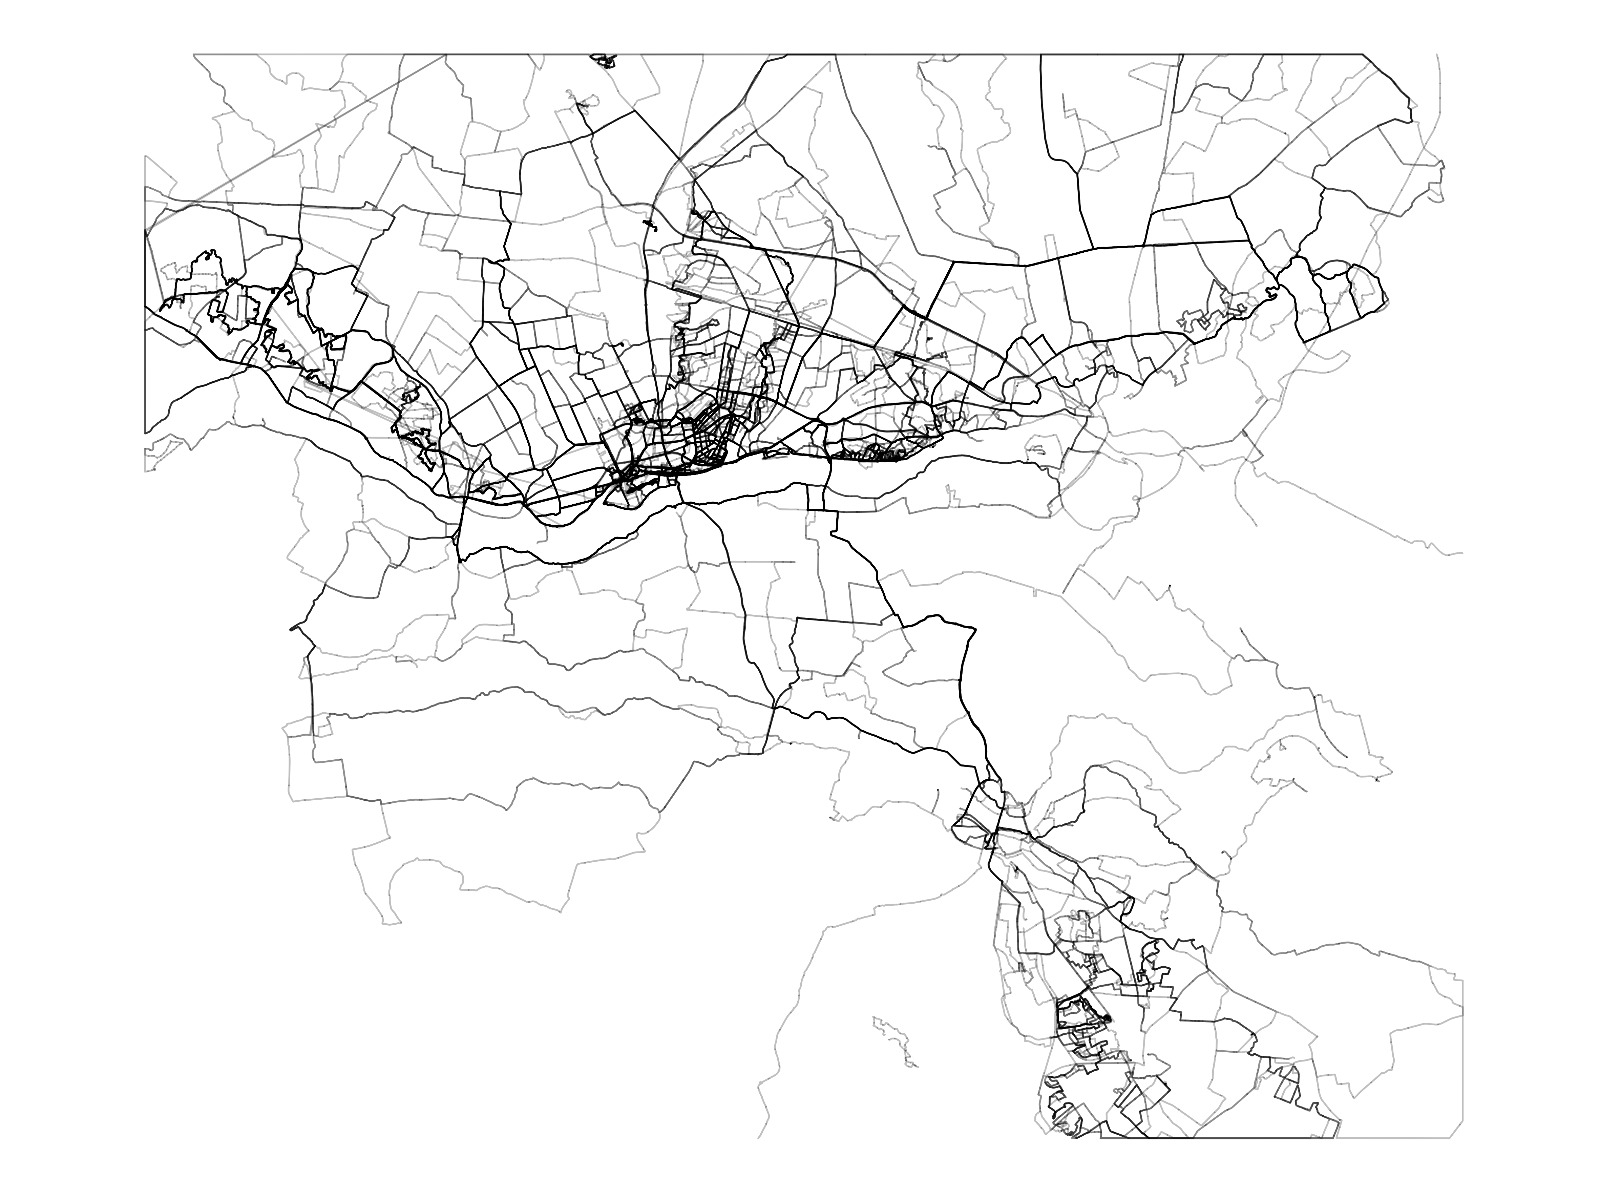
\includegraphics[width=0.78\textwidth]{Figures/Fig2}
\caption{\textbf{In vivo cleavage assay. }\textbf{a)} gRNAs 1, 2, and 3 with Avr1 as target DNA. \textbf{b)} gRNA8 with PiTubA2 as target DNA (\textbf{right}) and gRNA183 with PiAP5 as target DNA (\textbf{left}).}
\label{fig2_cleaving}
\end{figure*}

\subsection{Experiment 4}
\lipsum[1]

\subsubsection{Sub experiment a}
\lipsum[1]

\subsubsection{Sub experiment b}
\lipsum[1]

\subsubsection{Sub experiment c}
\lipsum[1]

\section{Discussion}
\lipsum[1-6]

\section{Acknowledgements}
We are grateful to our colleagues who generously shared their constructs and experiences. This work was supported by xxx with financial aid from the xxx in the framework of the xxx programme (project \# 1234).

\begin{footnotesize}
\section{Materials and methods}

\subsection{Culturing conditions}
\lipsum[1]

\subsection{Experimental procedures}
\lipsum[1]

\subsection{Constructs}
\lipsum[1]

\subsection{Cas9 \textit{in vitro} activity assay}
\lipsum[1]

\subsection{Molecular analysis of transformants}
\lipsum[1]

\subsection{T7EI assay}
\lipsum[1]

\section{Data availability}
All data is public available under xxx.

\end{footnotesize}


\section{References}
\setlength\parindent{-0.5 em}
\setlength{\parskip}{0 em}
\setlength{\leftskip}{0.5 em}

\begin{sloppy}
\begin{footnotesize}
Ah-Fong, A. M., C. A. Bormann-Chung and H. S. Judelson (2008). Optimization of transgene-mediated silencing in \textit{Phytophthora infestans} and its association with small-interfering RNAs, \textit{Fungal Genet Biol} \textbf{45}: 1197-1205. doi: 10.1016/j.fgb.2008.05.009

Ah-Fong, A. M. and H. S. Judelson (2011). Vectors for fluorescent protein tagging in \textit{Phytophthora}: tools for functional genomics and cell biology, \textit{Fungal Biol} \textbf{115}: 882-890. doi: 10.1016/j.funbio.2011.07.001

Brinkman, E. K., T. Chen, M. Amendola and B. van Steensel (2014). Easy quantitative assessment of genome editing by sequence trace decomposition, \textit{Nucleic Acids Res} \textbf{42}: e168. doi: 10.1093/nar/gku936

Caten, C. E. and J. L. Jinks (1968). Spontaneous Variability of Single Isolates of \textit{Phytophthora infestans}. Cultural Variation, \textit{Can J Botany} \textbf{46}: 329-348. doi: 10.1139/b68-055

Chen, F., S. M. Pruett-Miller, Y. Huang, M. Gjoka, K. Duda, J. Taunton, . . . G. D. Davis (2011). High-frequency genome editing using ssDNA oligonucleotides with zinc-finger nucleases, \textit{Nat Methods} \textbf{8}: 753-755. doi: 10.1038/nmeth.1653

Cho, S. W., J. Lee, D. Carroll, J. S. Kim and J. Lee (2013). Heritable gene knockout in \textit{Caenorhabditis elegans} by direct injection of Cas9-sgRNA ribonucleoproteins, \textit{Genetics} \textbf{195}: 1177-1180. doi: 10.1534/genetics.113.155853

Doench, J. G., E. Hartenian, D. B. Graham, Z. Tothova, M. Hegde, I. Smith, . . . D. E. Root (2014). Rational design of highly active sgRNAs for CRISPR-Cas9-mediated gene inactivation, \textit{Nat Biotechnol} \textbf{32}: 1262-1267. doi: 10.1038/nbt.3026

Du, Y., R. Weide, Z. Zhao, P. Msimuko, F. Govers and K. Bouwmeester (2018). RXLR effector diversity in Phytophthora infestans isolates determines recognition by potato resistance proteins; the case study AVR1 and R1, \textit{Studies in Mycology}. doi: 10.1016/j.simyco.2018.01.003

Edvardsen, R. B., S. Leininger, L. Kleppe, K. O. Skaftnesmo and A. Wargelius (2014). Targeted mutagenesis in Atlantic salmon (\textit{Salmo salar L.}) using the CRISPR/Cas9 system induces complete knockout individuals in the F0 generation, \textit{PLoS One} \textbf{9}: e108622. doi: 10.1371/journal.pone.0108622

Fang, Y., H. S. Jang, G. W. Watson, D. P. Wellappili and B. M. Tyler (2017). Distinctive Nuclear Localization Signals in the Oomycete \textit{Phytophthora sojae}, \textit{Front Microbiol} \textbf{8}: 10. doi: 10.3389/fmicb.2017.00010

Fang, Y. and B. M. Tyler (2016). Efficient disruption and replacement of an effector gene in the oomycete \textit{Phytophthora sojae} using CRISPR/Cas9, \textit{Mol Plant Pathol} \textbf{17}: 127-139. doi: 10.1111/mpp.12318

Fry, W. (2008). \textit{Phytophthora infestans}: the plant (and R gene) destroyer, \textit{Mol Plant Pathol} \textbf{9}: 385-402. doi: 10.1111/j.1364-3703.2007.00465.x

Gamboa-Melendez, H., A. I. Huerta and H. S. Judelson (2013). bZIP transcription factors in the oomycete \textit{Phytophthora infestans} with novel DNA-binding domains are involved in defense against oxidative stress, \textit{Eukaryot Cell} \textbf{12}: 1403-1412. doi: 10.1128/EC.00141-13

Govers, F. and M. Gijzen (2006). \textit{Phytophthora }genomics: the plant destroyers' genome decoded, \textit{Mol Plant Microbe Interact} \textbf{19}: 1295-1301. doi: 10.1094/MPMI-19-1295

Grahl, N., E. G. Demers, A. W. Crocker and D. A. Hogan (2017). Use of RNA-Protein Complexes for Genome Editing in Non-albicans \textit{Candida} Species, \textit{mSphere} \textbf{2}. doi: 10.1128/mSphere.00218-17

Gumtow, R., D. Wu, J. Uchida and M. Tian (2017). A \textit{Phytophthora palmivora} extracellular cystatin-like protease inhibitor targets papain to contribute to virulence on papaya, \textit{Mol Plant Microbe Interact}. doi: 10.1094/MPMI-06-17-0131-FI

Haas, B. J., S. Kamoun, M. C. Zody, R. H. Jiang, R. E. Handsaker, L. M. Cano, . . . C. Nusbaum (2009). Genome sequence and analysis of the Irish potato famine pathogen \textit{Phytophthora infestans}, \textit{Nature} \textbf{461}: 393-398. doi: 10.1038/nature08358

Hsu, P. D., D. A. Scott, J. A. Weinstein, F. A. Ran, S. Konermann, V. Agarwala, . . . F. Zhang (2013). DNA targeting specificity of RNA-guided Cas9 nucleases, \textit{Nat Biotechnol} \textbf{31}: 827-832. doi: 10.1038/nbt.2647

Jiang, W., A. J. Brueggeman, K. M. Horken, T. M. Plucinak and D. P. Weeks (2014). Successful transient expression of Cas9 and single guide RNA genes in \textit{Chlamydomonas reinhardtii}, \textit{Eukaryot Cell} \textbf{13}: 1465-1469. doi: 10.1128/EC.00213-14

Judelson, H. and B. M. Tyler. (2001). "Transformation of \textit{Phytohpthora infestans }by electroporation." from https://oomyceteworld.net/Phytophthora electroporatio.pdf.

Judelson, H. S. (1997). The genetics and biology of \textit{Phytophthora infestans}: modern approaches to a historical challenge, \textit{Fungal Genet Biol} \textbf{22}: 65-76. doi: 10.1006/fgbi.1997.1006

Kamoun, S., O. Furzer, J. D. Jones, H. S. Judelson, G. S. Ali, R. J. Dalio, . . . F. Govers (2015). The Top 10 oomycete pathogens in molecular plant pathology, \textit{Mol Plant Pathol} \textbf{16}: 413-434. doi: 10.1111/mpp.12190

Kay, J., H. J. G. Meijer, A. ten Have and J. A. van Kan (2011). The aspartic proteinase family of three \textit{Phytophthora }species, \textit{BMC Genomics} \textbf{12}: 254. doi: 10.1186/1471-2164-12-254

Kearse, M., R. Moir, A. Wilson, S. Stones-Havas, M. Cheung, S. Sturrock, . . . A. Drummond (2012). Geneious Basic: an integrated and extendable desktop software platform for the organization and analysis of sequence data, \textit{Bioinformatics} \textbf{28}: 1647-1649. doi: 10.1093/bioinformatics/bts199

Kim, S., D. Kim, S. W. Cho, J. Kim and J. S. Kim (2014). Highly efficient RNA-guided genome editing in human cells via delivery of purified Cas9 ribonucleoproteins, \textit{Genome Res} \textbf{24}: 1012-1019. doi: 10.1101/gr.171322.113

Kleinstiver, B. P., S. Q. Tsai, M. S. Prew, N. T. Nguyen, M. M. Welch, J. M. Lopez, . . . J. K. Joung (2016). Genome-wide specificities of CRISPR-Cas Cpf1 nucleases in human cells, \textit{Nat Biotechnol} \textbf{34}: 869-874. doi: 10.1038/nbt.3620

Lange, A., R. E. Mills, C. J. Lange, M. Stewart, S. E. Devine and A. H. Corbett (2007). Classical nuclear localization signals: definition, function, and interaction with importin alpha, \textit{J Biol Chem} \textbf{282}: 5101-5105. doi: 10.1074/jbc.R600026200

Le Blanc, C., F. Zhang, J. Mendez, Y. Lozano, K. Chatpar, V. Irish and Y. Jacob (2017). Increased efficiency of targeted mutagenesis by CRISPR/Cas9 in plants using heat stress, \textit{Plant J}. doi: 10.1111/tpj.13782

Ma, Z., L. Zhu, T. Song, Y. Wang, Q. Zhang, Y. Xia, . . . Y. Wang (2017). A paralogous decoy protects \textit{Phytophthora sojae} apoplastic effector PsXEG1 from a host inhibitor, \textit{Science} \textbf{355}: 710-714. doi: 10.1126/science.aai7919

Peng, D., S. P. Kurup, P. Y. Yao, T. A. Minning and R. L. Tarleton (2014). CRISPR-Cas9-mediated single-gene and gene family disruption in \textit{Trypanosoma cruzi}, \textit{mBio} \textbf{6}: e02097-02014. doi: 10.1128/mBio.02097-14

Pohl, C., J. A. Kiel, A. J. Driessen, R. A. Bovenberg and Y. Nygard (2016). CRISPR/Cas9 Based Genome Editing of \textit{Penicillium chrysogenum}, \textit{ACS Synth Biol} \textbf{5}: 754-764. doi: 10.1021/acssynbio.6b00082

Poidevin, L., K. Andreeva, C. Khachatoorian and H. S. Judelson (2015). Comparisons of Ribosomal Protein Gene Promoters Indicate Superiority of Heterologous Regulatory Sequences for Expressing Transgenes in \textit{Phytophthora infestans}, \textit{PLoS One} \textbf{10}: e0145612. doi: 10.1371/journal.pone.0145612

Ramakrishna, S., A. B. Kwaku Dad, J. Beloor, R. Gopalappa, S. K. Lee and H. Kim (2014). Gene disruption by cell-penetrating peptide-mediated delivery of Cas9 protein and guide RNA, \textit{Genome Res} \textbf{24}: 1020-1027. doi: 10.1101/gr.171264.113

Ran, F. A., L. Cong, W. X. Yan, D. A. Scott, J. S. Gootenberg, A. J. Kriz, . . . F. Zhang (2015). In vivo genome editing using Staphylococcus aureus Cas9, \textit{Nature} \textbf{520}: 186-191. doi: 10.1038/nature14299

Ran, F. A., P. D. Hsu, J. Wright, V. Agarwala, D. A. Scott and F. Zhang (2013). Genome engineering using the CRISPR-Cas9 system, \textit{Nat Protoc} \textbf{8}: 2281-2308. doi: 10.1038/nprot.2013.143

Reuter, J. S. and D. H. Mathews (2010). RNAstructure: software for RNA secondary structure prediction and analysis, \textit{BMC Bioinformatics} \textbf{11}: 129. doi: \mbox{10.1186/1471-2105-11-129}

Soares Medeiros, L. C., L. South, D. Peng, J. M. Bustamante, W. Wang, M. Bunkofske, . . . R. L. Tarleton (2017). Rapid, Selection-Free, High-Efficiency Genome Editing in Protozoan Parasites Using CRISPR-Cas9 Ribonucleoproteins, \textit{mBio} \textbf{8}. doi: 10.1128/mBio.01788-17

Stajich, J. E., T. Harris, B. P. Brunk, J. Brestelli, S. Fischer, O. S. Harb, . . . D. S. Roos (2012). FungiDB: an integrated functional genomics database for fungi, \textit{Nucleic Acids Res} \textbf{40}: D675-681. doi: 10.1093/nar/gkr918

Van den Hoogen, D. J., H. J. G. Meijer, M. F. Seidl and F. Govers (2018). The ancient link between G-protein coupled receptors and C-terminal phospholipid kinase domains, \textit{mBio} \textbf{9}. doi: 10.1128/mBio.02119-17

van der Lee, T., A. Robold, A. Testa, J. W. van 't Klooster and F. Govers (2001). Mapping of avirulence genes in \textit{Phytophthora infestans} with amplified fragment length polymorphism markers selected by bulked segregant analysis, \textit{Genetics} \textbf{157}: 949-956. 

van West, P., S. Kamoun, J. W. van 't Klooster and F. Govers (1999). Internuclear gene silencing in Phytophthora infestans, \textit{Mol Cell} \textbf{3}: 339-348.

Verdonk, J. (2014). RNA isolation with homemade TRIzol reagent. from https://julianverdonk.wordpress.com/2014/01/14/rna-isolation-with-homemade-trizol-reagent/.

Vijn, I. and F. Govers (2003). Agrobacterium tumefaciens mediated transformation of the oomycete plant pathogen Phytophthora infestans, \textit{Mol Plant Pathol} \textbf{4}: 459-467. doi: 10.1046/j.1364-3703.2003.00191.x

Woo, J. W., J. Kim, S. I. Kwon, C. Corvalan, S. W. Cho, H. Kim, . . . J. S. Kim (2015). DNA-free genome editing in plants with preassembled CRISPR-Cas9 ribonucleoproteins, \textit{Nat Biotechnol} \textbf{33}: 1162-1164. doi: 10.1038/nbt.3389

\end{footnotesize}
\end{sloppy}
\end{multicols}

\clearpage

\section{Supplementary files}
\makeatletter 
\setcounter{figure}{0}
\renewcommand{\thetable}{S\arabic{table}}   
\renewcommand{\thefigure}{S\arabic{figure}}
\renewcommand{\figurename}{Supplemental Figure}
\renewcommand{\tablename}{Supplemental Table}

\begin{figure*}[h]
\centering
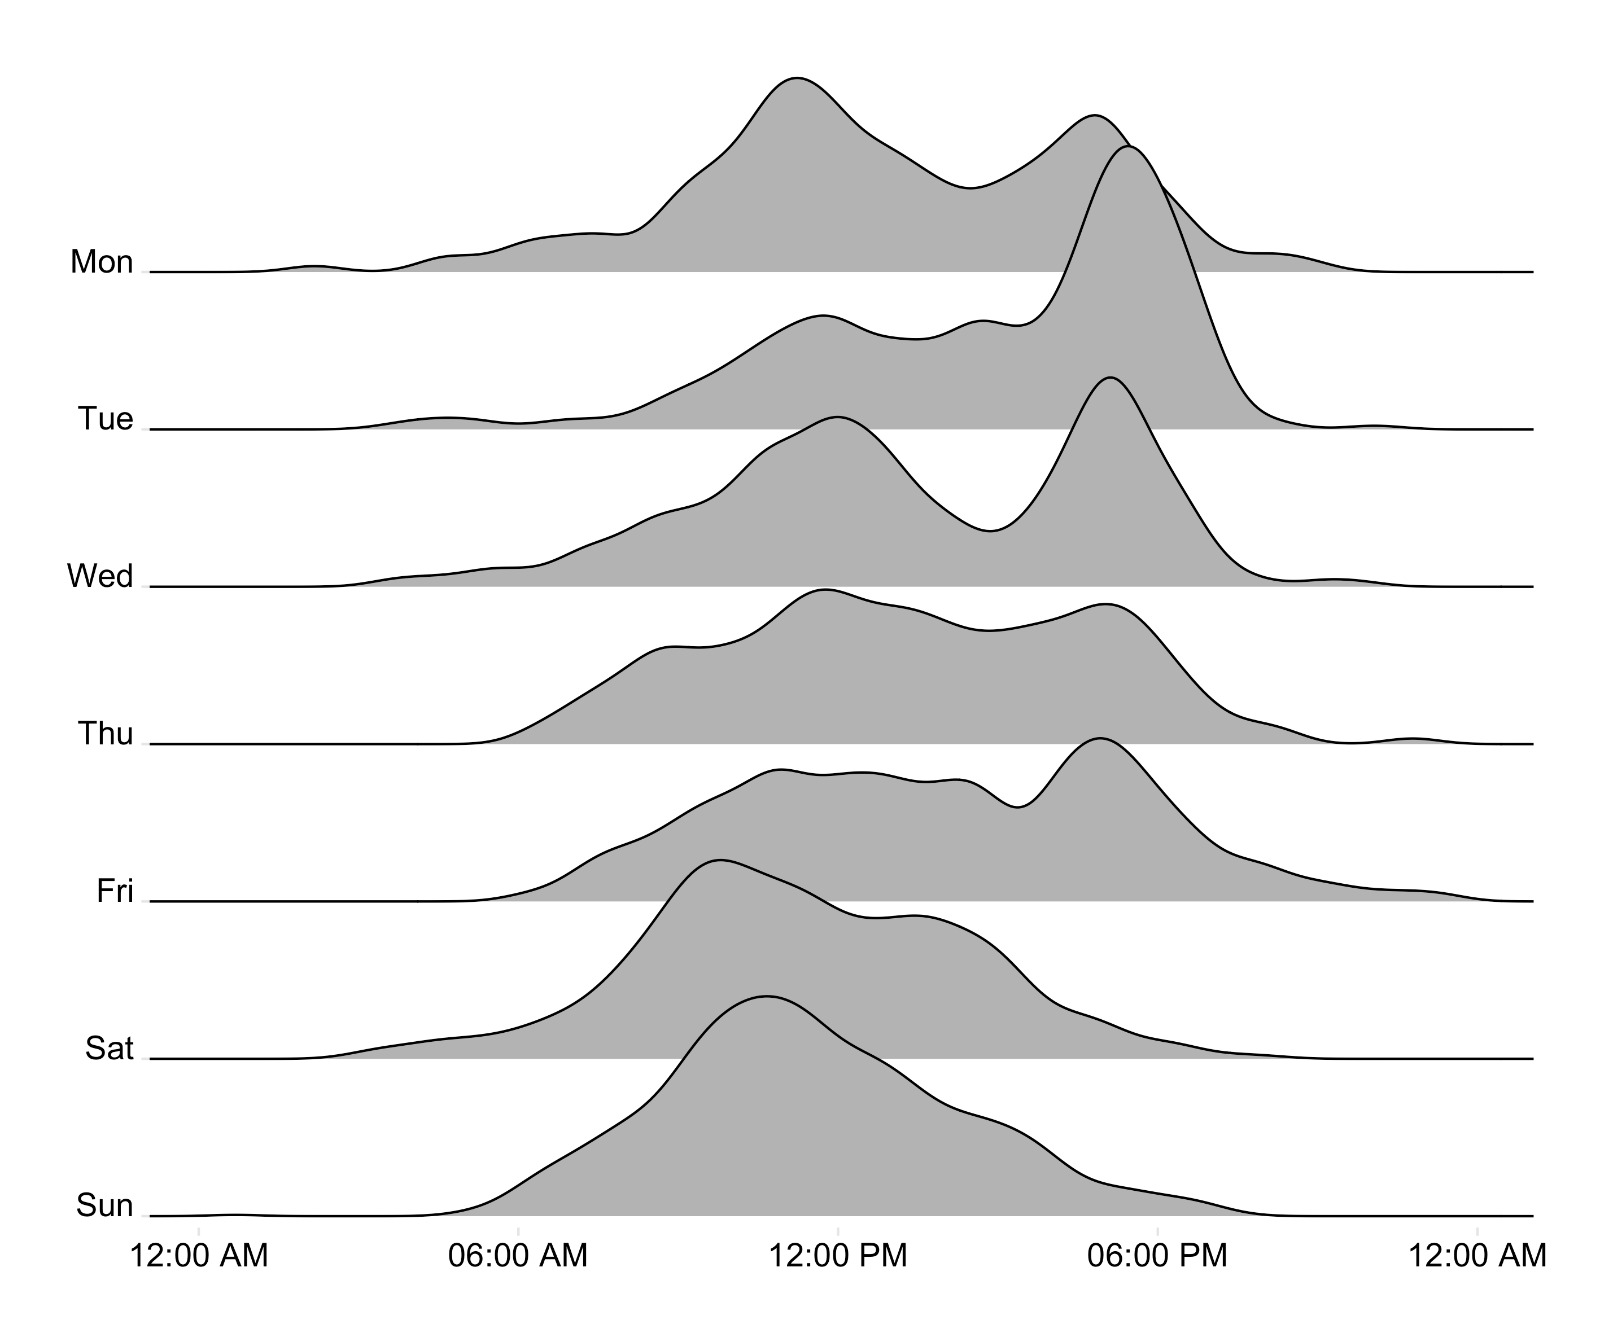
\includegraphics[width=0.7\textwidth]{Figures/FigS1}
\caption{\textbf{Detection limit assays.} \textbf{a)} PCR amplicons used for the detection limit assays. ΔAvr1 contains a 29 bp deletion. \textbf{b)} T7EI assay. Varying amounts of Avr1 and ΔAvr1 PCR amplicons were annealed and digested by T7EI. \textbf{c)} Example output from TIDE, confirming the presence of the 29 bp deletion in ΔAvr1 (left red bar). Here, a sequence chromatogram obtained from sequencing a molar ratio of 998:2 Avr1:ΔAvr1 was compared to a sequence chromatogram of Avr1. The predicted frequency of chromatograms with a deletion (1.5\%) deviates from the actual molar ratio of Avr1:ΔAvr1 (0.2\%).}
\label{figS1_detect}
\end{figure*}

\begin{figure*}[h]
\centering
\includegraphics[width=\textwidth]{Figures/FigS2}
\caption{\textbf{Expression analysis of Cas9 in 11 selected transformed lines.} cDNA and genomic DNA (gDNA) of\textit{ P. infestans }strain T30-2 were used as negative control and gDNA from a \textit{P. infestans} Cas9 transformant as positive control.}
\label{figS2_RT}
\end{figure*}

\begin{figure*}[h]
\centering
\includegraphics[width=\textwidth]{Figures/FigS3}
\caption{\textbf{Plasmids used in this study.} Plasmids starting with `pYF' are obtained from Francis Fang (Fang \& Tyler 2017), plamids starting with `pJH' are modified versions as described in this report.}
\label{figS3_Plasmids}
\end{figure*}

\begin{table*}[h]
\rowcolors{0}{}{lightgray}
\centering
\caption{\textbf{Primers used in this study}.}
\label{TabS1_primers}
\resizebox{\textwidth}{!}{%
\begin{tabular}{llll}
\hline
\textbf{Name}                     & \textbf{Sequence (5' - 3')}                           & \textbf{Purpose}                                   &  \\ \hline
Avr1\_F                  & ATGCACCGCGTATTGCTGC                          & \textit{P. infestans} T30-2 Avr1          &  \\
Avr1\_F                  & TTAAAATGGTACCACAACATGTCCACC                  & \textit{P. infestans} T30-2 Avr1          &  \\
Avr1\_Nested F           & GACGTTTGCCCTGTTGTGTA                         & \textit{P. infestans} T30-2 Avr1 - nested &  \\
Avr1\_Nested R           & ACAACATGTCCACCAAGCATG                        & \textit{P. infestans} T30-2 Avr1 - nested &  \\
pRPL41\_seq\_F           & CAAGCCTCACTTTCTGCTGACTG                      & Sequence analysis of gRNA constructs      &  \\
sgRNA\_Col\_R            & AAAAGCACCGACTCGGTGC                          & Sequence analysis of gRNA constructs      &  \\
Cas9\_RT\_F              & CCGAAGAGGTCGTGAAGAAG                         & Expression analysis of Cas9               &  \\
Cas9\_RT\_R              & GCCTTATCCAGTTCGCTCAG                         & Expression analysis of Cas9               &  \\
pHAM34\_Pseq\_F          & TCGCCCGACTCGCCCAC                            & Sequence analysis of Cas9                 &  \\
Cas9\_Seq\_757\_F        & CTGTTCGGAAACCTGATTGCCC                       & Sequence analysis of Cas9                 &  \\
Cas9\_Seq\_1439\_F       & GGATGACCAGAAAGAGCGAGG                        & Sequence analysis of Cas9                 &  \\
Cas9\_Seq\_2163\_F       & AGAGGACATCCAGAAAGCCCAGG                      & Sequence analysis of Cas9                 &  \\
Cas9\_Seq\_2865\_F       & GAACACTAAGTACGACGAGAATGAC                    & Sequence analysis of Cas9                 &  \\
Cas9\_Seq\_3600\_F       & CAAGGGCTACAAAGAAGTGAAAAAG                    & Sequence analysis of Cas9                 &  \\
eGFP\_F                  & ATGGGCAAGGGCGAGGAA                           & Detection of eGFP                         &  \\
eGFP\_R                  & TCACTTGTAGAGTTCATCCATGCCA                    & Detection of eGFP                         &  \\
Hyg\_ApaI\_R             & GGGCCCCTATTCCTTTGCCCTC                       & Cloning Hygromycin into pYF2.3            &  \\
Hyg-AflII\_F             & CTTAAGATGAAAAAGCCTGAACTCAC                   & Cloning Hygromycin into pYF2.3            &  \\
M13F                     & CGTTGTAAAACGACGGCCAG                         & General primers                           &  \\
M13R                     & TGCCAGGAAACAGCTATGACC                        & General primers                           &  \\
PiNLS\_SacII\_F          & ACACCCGCGGATGCACAAGCGCAAG                    & Cloning PiNLS in pYF2.2                   &  \\
PiNLS\_SpeI\_R           & ACACACTAGTCTCGCCCATTGCCGCGTC                 & Cloning PiNLS in pYF2.2                   &  \\
PiNLS\_AgeI\_F           & ACACACCGGTATGCACAAGCGCAAG                    & Cloning PiNLS in pGFPN                    &  \\
PiNLS\_NheI\_R           & ACACGCTAGCCTCGCCCATTGCCGCGTC                 & Cloning PiNLS in pGFPN                    &  \\
PiAP5\_EcoRI\_F          & ACACGAATTCATGCGTCTCGGTCTGCTC                 & PiAp5 full-length                         &  \\
PiAP5\_NotI\_R           & ACACGCGGCCGCATTTGGTCCCATGAGACGCG             & PiAp5 full-length                         &  \\
PcS9\_F\_EcoRI           & cacaGAATTCCGTCAATACGGCTGTAAACCAC             & \textit{P. capsici S9} promoter          &  \\
PcS9\_F\_NheI            & cacaGCTAGCTTTGGCGACTTCTTTTGTTCAGG            & \textit{P. capsici S9} promoter           &  \\
Avr1\_gRNA\_1\_pT7\_F    & GAAATTAATACGACTCACTATAGGTGGCCAAAGCAATGATATTG & In vitro transcription gRNA               &  \\
Avr1\_gRNA\_2\_pT7\_F    & GAAATTAATACGACTCACTATAGGTCGTTTATCGAGTCCTTCGT & In vitro transcription gRNA               &  \\
Avr1\_gRNA\_3\_pT7\_F    & GAAATTAATACGACTCACTATAGGGAATCCAAGACTCGATTTTT & In vitro transcription gRNA               &  \\
PiTubA2\_gRNA\_8\_pT7\_F & GAAATTAATACGACTCACTATAGGACGCATGTTGCTTTAAGCTT & In vitro transcription gRNA               &  \\
PiAP5\_gRNA\_183\_pT7\_F & GAAATTAATACGACTCACTATAGGGATAAGACGGTGAACAGCAA & In vitro transcription gRNA               &  \\
gRNA3\_Gibson\_F         & TCGGCATGGCGAATGGGACAGGATTCCTGATGAGTCCGTGA    & gRNA2-3 plasmid assembly                   &  \\
gRNA3\_Gibson\_R         & GCTAAGTATTCTAGTCGACAGTCCCATTCGCCATGCCGAA     & gRNA2-3 plasmid assembly                           &  \\ \hline
\end{tabular}%
}
\end{table*}

\end{document}